% Template for ICASSP-2013 paper; to be used with:
%          spconf.sty  - ICASSP/ICIP LaTeX style file, and
%          IEEEbib.bst - IEEE bibliography style file.
% --------------------------------------------------------------------------
\documentclass{article}
\usepackage{spconf,amsmath,graphicx}
\usepackage{graphicx}
\usepackage{cite}
\usepackage{url}
\usepackage{hyperref}
\usepackage{cleveref}
\usepackage{booktabs}
\usepackage{brian}

% Title.
% ------
\title{Better beat tracking through robust onset aggregation}
%
% Single address.
% ---------------
% \name{Author Names\thanks{Thanks to XYZ agency for funding.}}
% \address{Author Affiliations}
%
% For example:
% ------------
%\address{School\\
%   Department\\
%   Address}
%
% Two addresses (uncomment and modify for two-address case).
% ----------------------------------------------------------
\twoauthors%
 {Brian McFee\thanks{This work was supported by a grant from the Mellon foundation, and
grant IIS-1117015 from the National Science Foundation (NSF).}}{ Center for Jazz Studies\\
      Columbia University\\
  \texttt{brm2132@columbia.edu}}%
 {Daniel P.W. Ellis}{
  LabROSA, Department of Electrical Engineering\\
      Columbia University\\
  \texttt{dpwe@columbia.edu}}
%
\begin{document}
%\ninept
%
\maketitle
%
\begin{abstract}
Onset detection forms the critical first stage of most beat tracking algorithms.
While common spectral-difference onset detectors can work well in genres with clear 
rhythmic structure, they can be sensitive to loud, asynchronous events (\eg, off-beat 
notes in a jazz solo), which limits their general efficacy. In this paper, we investigate 
methods to improve the robustness of onset detection for beat tracking. 
Experimental results indicate that simple modifications to onset detection can produce
large improvements in beat tracking accuracy.
\end{abstract}
%
\begin{keywords}
Music information retrieval, beat tracking
\end{keywords}
%
\section{Introduction}
\label{sec:intro}
Beat-tracking --- the detection of ``pulse'' or salient, rhythmic events in a musical 
performance --- is a fundamental problem in music content analysis. Automatic 
beat-detection methods are often used for chord recognition, cover song detection, 
structural segmentation, transcription, and numerous other applications. A large body of 
literature has developed over the past two decades, and each year sees numerous 
submissions to the Music Information Retrieval Evaluation eXchange (MIREX) beat tracking 
evaluation~\cite{Downie2008}.

A common general strategy for beat tracking operates in two stages.  First, the 
audio signal is processed by an onset strength function, which measures the likelihood 
that a musically salient change (\eg, note onset) has occurred at each time point.  
The tracking algorithm then selects the beat times from among the peaks of the onset 
strength profile.

% FIXME:  2013-10-17 17:20:33 by Brian McFee <brm2132@columbia.edu>
%  Clean this up
As we will demonstrate, the behavior of standard onset detectors tends to be dominated by 
the loudest events, typically produced by predominant or foreground instruments and 
performers.  In many styles of western, popular music --- \eg, rock, dance, or pop --- 
this presents no difficulty. Often, the beat is unambiguously driven by percussion or 
foreground instrumentation, resulting in clear rhythmic patterns which are amenable 
to signal analysis. 
% As a result, beat detection in these genres is easily solved by prior 
% work.

The assumption that beat derives from the predominant foreground instrumentation does not 
hold in general across diverse categories of music. As a concrete example, a soloist in a 
jazz combo may play a syncopated rhythm, or off-beat for aesthetic or expressive purposes, 
while the accompaniment maintains a steady pulse in the background.  
In such cases, we would hope that a beat tracker would adaptively tune out the foreground 
instrumentation and focus on the rhythmically salient portion of the signal.

Reliable detection and separation of rhythmic elements in a recording can be quite
difficult to achieve in practice.  Humans can tap along to a
performance and adapt to sudden changes in instrumentation (\eg, a drum solo), but 
this behavior is difficult for an algorithm to emulate.

\subsection{Our contributions}
In this work, we investigate two complementary techniques to improve the robustness of 
beat tracking and onset detection. 
First, we propose across-frequency median onset aggregation, which captures temporally synchronous onsets, and is robust to spurious, large spectral deviations.
Second, we examine two spectrogram decomposition methods to separate the signal into distinct components, allowing the onset detector to suppress noisy or arrhythmic events. 

\section{Related work}
\label{sec:related}
Onset detection is a well-studied problem in music information retrieval, and a full
summary of recent work on the subject lies well beyond the scope of this paper.
Within the context of beat-tracking, the surveys by Bello \etal~\cite{bello2005tutorial}
and Collins~\cite{collins2005comparison} provide general introductions to the topic, and
evaluate a wide variety of different approaches to detecting onset events.  

Escalona-Espinosa applied harmonic-percussive separation to beat-tracking, and derived beat 
times from the self-similarity over features extracted from the different 
components~\cite{escalona2008downbeat}.  The approach taken in this work is rather
different, as we evaluate onset detectors derived from a single component of a
spectrogram decomposition.

Peeters~\cite{peeters2005time} and Wu \etal~\cite{wu2011two} highlight tempo variation as a 
key challenge in beat tracking. While tempo variation is indeed a challenge, our focus here 
is on improving the detection of salient onset events; the tracking algorithm used in
this work maintains a fixed tempo estimate for the duration of the track, but allows for
deviation from the tempo.

Alonso \etal~\cite{alonso2004tempo} and Bello \etal~\cite{bello2005tutorial} propose using 
temporal median-filtering of the onset strength envelope to reduce noise and suppress
spurious onset events.  Temporal smoothing differs from the median-aggregation method 
proposed in this work, which instead filters across frequencies at each time step prior to
constructing the onset envelope.

This article addresses the early stages of beat tracking.  Rather
than develop a new framework from scratch, we chose to modify the method
proposed by Ellis~\cite{ellis2007beat}, which operates in three stages:
\begin{enumerate}\addtolength{\itemsep}{-0.60\baselineskip}
\item compute an onset strength envelope $\omega(t)$,
\item estimate the tempo by picking peaks in the windowed auto-correlation of $\omega(t)$,
and
\item select beats consistent with the estimated tempo from the peaks of $\omega(t)$ by 
dynamic programming.
\end{enumerate}
Keeping steps 2--3 fixed allows us to evaluate the contribution to accuracy due to the
choice of onset strength function.
We expect that improvements to onset detection can be applied to benefit other beat
tracking architectures.

\section{Median onset aggregation}
\label{sec:onsets}

\begin{figure}
\centering%
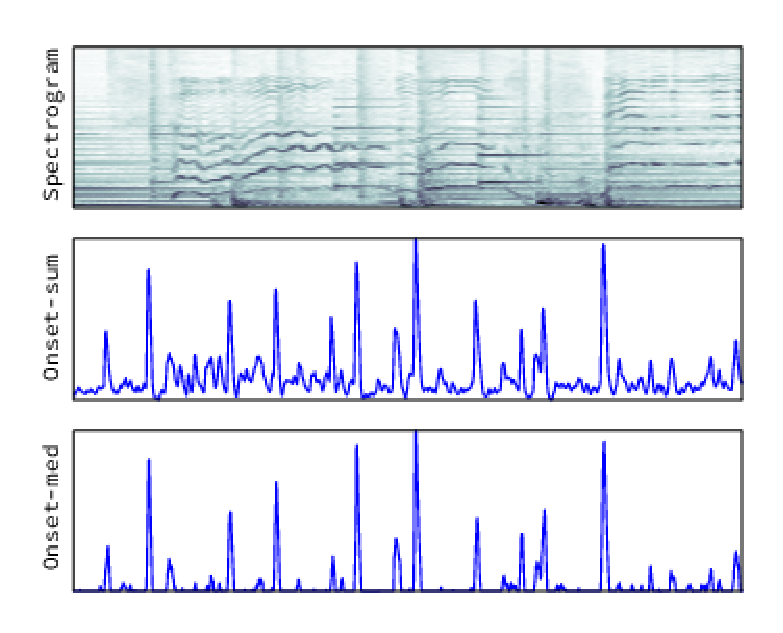
\includegraphics[width=\columnwidth]{figs/onsets}%
\vspace{-\baselineskip}
\caption{An example spectrogram (top) derived from five seconds of vocals, piano, and drums.  
Sum across frequency bands to derive onset strength (middle) results in spurious peaks due to vibrato.
Median aggregation (bottom) produces a sparser onset strength function, and retains the salient peaks.}
\label{fig:onsets}
\end{figure}

The general class of onset detector functions we consider is based on \emph{spectral 
difference}, \ie, measuring the change in spectral energy across frequency bands in 
successive spectrogram frames~\cite{bello2005tutorial}. The tracker 
of Ellis~\cite{ellis2007beat} uses the sum across bands of thresholded log-magnitude
difference to determine the onset strength at time $t$:
\begin{equation}
\omega_s(t) \defeq \sum_f \max(0, \log S_{f, t} - \log S_{f, t-1}),\label{eq:onset:sum}
\end{equation}
where $S \in \R_+^{d\times T}$ denotes the (Mel-scaled) magnitude spectrogram.  
This function effectively measures increasing spectral energy over time across 
\emph{any} frequency band $f$, and its magnitude scales in proportion to the 
difference.

Note that $\omega_s$ can respond equally to either a large fluctuation confined to a 
single frequency band, or many small fluctuations spread across multiple frequency bands.
The latter case typically arises from either a percussive event or multiple synchronized 
note onset events, both of which can be strong indicators of a beat.  However, the former 
case can only arise when a single source plays out of sync with the other sources, such 
as a vocalist coming in late for dramatic effect.

To better capture temporally synchronous onset events, we propose to replace the sum
across frequency bands with the median operator:
\begin{equation}
\omega_m(t) \defeq \median_f \max(0, \log S_{f, t} - \log S_{f, t-1}).\label{eq:onset:median}
\end{equation}
This simple modification improves the robustness of the onset strength function to loud, 
asynchronous events.  The resulting onset envelope tends to be sparser, since it can only 
produce non-zero values if more than half of the frequency bins increase in energy 
simultaneously.\footnote{In preliminary experiments, alternative quantile estimators 
(25th and 75th percentile) were found to be inferior to median aggregation.}

\section{Spectrogram decomposition}
\label{sec:spectrogram}

\begin{figure*}
\centering%
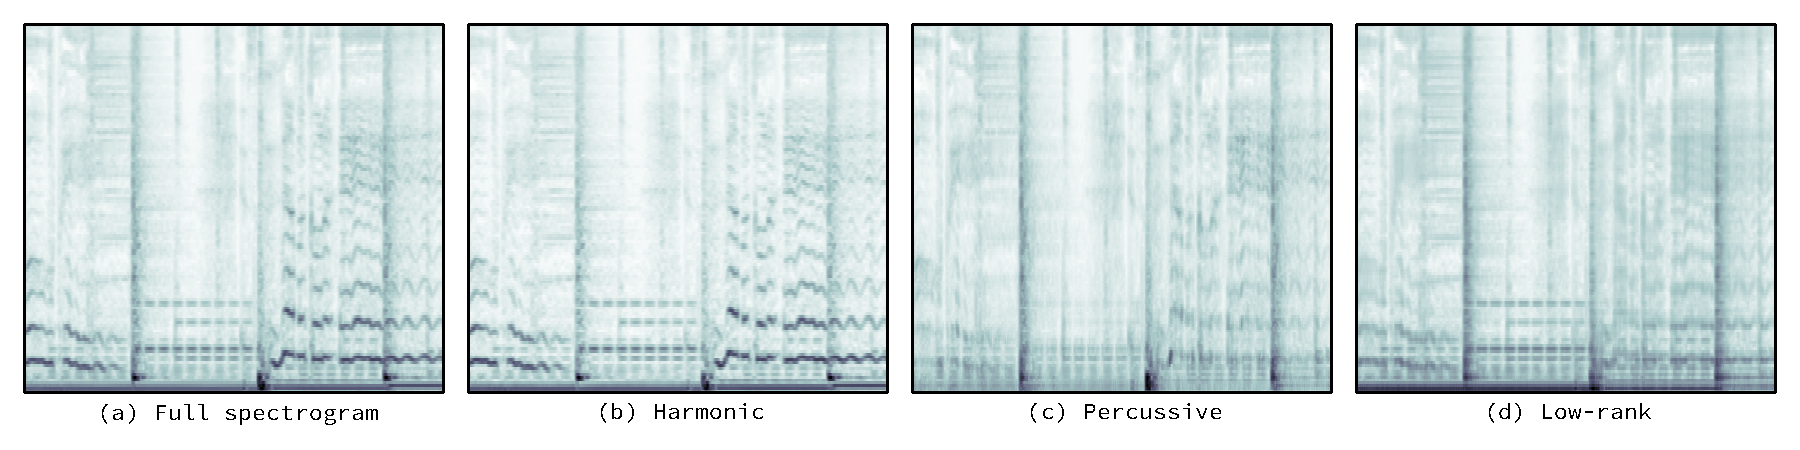
\includegraphics[width=\textwidth]{figs/specgrams}%
\vspace{-\baselineskip}%
\caption{Examples of each spectrogram decomposition method: 
(a) 6.5s of the original (Mel-scaled) spectrogram, consisting of guitar, bass, drums, and vocals; 
(b) the harmonic component emphasizes sustained tones (horizontal lines); 
(c) the percussive emphasizes transients (vertical lines); 
(d) the low-rank component retains horizontals and verticals, but suppresses vocals.}
\label{fig:specgrams}
\end{figure*}

In a typical musical recording, multiple instruments will play simultaneously. When
all instruments (generally, sound sources) are synchronized, computing onsets
directly from the spectrogram is likely to work well.  
However, if one or more sources play out of sync from each-other, it becomes difficult
to differentiate the rhythmically meaningful onsets from the off-beat events.  This
motivates the use of source separation techniques to help isolate the sources of beat
events.  In this work, we applied two different source-separation techniques which have
been demonstrated to work well for musical signals: harmonic-percussive source 
separation~\cite{ono2008real}, and robust principal components analysis~\cite{candes2011robust}.

\subsection{Harmonic-percussive source separation}
Harmonic-percussive source separation (HPSS) describes the general class of algorithms
which decompose the magnitude spectrogram as $S = H + P$, where $H$ denotes 
\emph{harmonics} --- sustained tones concentrated in a small set of frequency bands ---  
and $P$ denotes \emph{percussives} --- transients with broad-band 
energy~\cite{ono2008real}.  

In this work, we used the median-filtering method of 
Fitzgerald~\cite{fitzgerald2010harmonic}.  Let $\eta$ and $\pi$ denote the harmonic-
and percussive-enhanced spectrograms:
\begin{align*}
\pi  &\defeq \mathcal{M}(S, w_p, 1)\\
\eta &\defeq \mathcal{M}(S, 1, w_h),
\end{align*}
where $\mathcal{M}(\cdot, w_p, w_h)$ denotes a two-dimensional median filter with window 
size $w_p\times w_h$.
The percussive component $P$ is then recovered by soft-masking $S$:
\begin{align*}
P_{f,t} &= S_{f,t} \left(\frac{ \pi_{f,t}^p }{\pi_{f,t}^p + \eta_{f,t}^p}\right),
\end{align*}
where $p>0$ is a scaling parameter (typically $p=1$ or $2$). Given $P$, the harmonic 
component $H$ is recovered by ${H=S-P}$.

\Cref{fig:specgrams}~(a--c) illustrates an example of HPSS on a short song excerpt.
The harmonic component (b) retains most of the tonal content of the original signal (a),
while the percussive component (c) retains transients.

In the context of beat tracking, it may be reasonable to use either $H$ or $P$ as the
input spectrogram, depending on the particular instrumentation. While percussive
instruments reliably indicate the beat in many genres (rock, dance, pop, \etc), this
phenomenon is far from universal, particularly when the signal lacks percussion 
(\eg, a solo piano).

\subsection{Robust principal components analysis}
In contrast to a fixed decomposition (\ie, HPSS), it may be more effective to apply an
adaptive decomposition which exploits the structure of the spectrogram in question.
Recently, Yang demonstrated that robust principal components analysis (RPCA) can be
effective for separating vocals from accompanying instrumentation~\cite{yang2012sparse, 
candes2011robust}.  In this setting, RPCA finds a low-rank matrix $L \approx S$ which
approximates $S$ by solving the following convex optimization problem
\begin{equation}
L \leftarrow \argmin_L \|L\|_* + \lambda \|S - L\|_1,
\end{equation}
where $\|\cdot\|_*$ denotes the nuclear norm, $\|\cdot\|_1$ is the element-wise
1-norm, and $\lambda>0$ is a trade-off parameter.

In practice, the low-rank approximation tends to suppress pitch bends and vibrato,
which are both common characteristics of vocals and may account for some of its success
at vocal separation.  Pitch bends can trigger spurious onset 
detections due to lack of temporal continuity within each frequency band, and should
therefore be suppressed for beat tracking.  

\section{Evaluation}
\label{sec:eval}

To evaluate the proposed methods, we measured the alignment of detected beat events to 
beat taps generated by human annotators.  Following previous work, we report the
following standard beat tracking metrics~\cite{davies2009evaluation}:
\begin{description}\addtolength{\itemsep}{-.75\baselineskip}
\item[AMLt] (range: $[0, 1]$, larger is better) is a continuity-based metric that
resolves predicted beats at different allowed metrical levels (AML), and is therefore 
robust against doubling or halving of detected tempo;
\item[F-measure] (range: $[0,1]$, larger is better) measures the precision and recall of ground truth beat events by the predictor; 
\item[Information gain] (range: $[0, \cdot)$, larger is better) measures the mutual information (in bits) between the predicted beat sequence and the ground truth annotations.
\end{description}
Because different human annotators may produce beat sequences at
different levels of granularity for the same track, meter-invariant measures such as
AMLt and Information Gain are generally preferred; we include F-measure for
completeness.

Algorithms were evaluated on SMC Dataset2~\cite{holzapfel2012}, which contains 217
40-second clips from a wide range of genres and instrumentations (classical, chanson, 
blues, jazz, solo guitar, \etc).  This dataset was designed to consist primarily of 
difficult examples, and represents the most challenging publicly available dataset for beat
tracking evaluation.  We include comparisons to the best-performing methods reported by
Holzapfel \etal~\cite{holzapfel2012} --- Degara \etal~\cite{degara2012reliability}, B\"{o}ck and Schedl~\cite{bock2011enhanced}, and
Klapuri \etal~\cite{klapuri2006analysis} --- and to the original implementation described by
Ellis~\cite{ellis2007beat}.

\subsection{Implementation}
Each track was sampled at 22050Hz, and Mel-scaled magnitude spectrograms were computed 
with a Hann-windowed short-time Fourier transform with 2048 samples ($\approx93$ms), hop 
of 64 samples ($\approx3$ms), $d=128$ Mel bands, and a maximum frequency cutoff of 8000Hz.
The HPSS window sizes were set as $w_p = w_h = 19$, and the power parameter was set 
to $p=1.0$.
Following Cand\`{e}s \etal~\cite{candes2011robust}, the RPCA parameter was set to
${\lambda = \sqrt{T}}$, where $T$ denotes the number of frames.
All algorithms were implemented in Python using \texttt{librosa}.\footnote{\url{http://github.com/bmcfee/librosa/}}

\subsection{Results}

\Cref{tab:results:smc2} lists the average scores achieved by the proposed methods on
SMC Dataset2. 
We first observe the gap in performance between \emph{sum-Full} and 
Ellis~\cite{ellis2007beat}, which differ only in their choice of parameters: the 
original implementation used a lower sampling rate (8000Hz), smaller window (256 samples) 
and hop (32 samples, 4ms), and fewer Mel bands ($d=32$).\footnote{The present
implementation also includes a small constant timing correction, which improves 
performance for some metrics, but is known to not affect the information gain
score~\cite{davies2009evaluation}.}
Regardless of spectrogram decomposition method, all sum-based methods (first group of 
results) perform comparably well, and although there are slight degradations, each give 
a modest improvement over the original implementation.

Replacing sum onset aggregation with median aggregation (second group of results)
boosts performance uniformly: for each decomposition and each metric, median
aggregation only improves the score.  The largest improvement is observed on the
percussive-component, which achieved the lowest scores with sum aggregation, but the
highest with median. Indeed, the combination of median aggregation with the percussive
component outperforms the best-performing methods reported by Holzapfel~\etal{} for both 
the AMLt and Information Gain metrics, and is within the range of F-measure scores 
statistically equivalent to the best ($0.346$--$0.401$)~\cite{holzapfel2012}.

The RPCA method (Low-rank) did not yield improvements over either the full spectrogram or HPSS methods.
This may be due to the fact that the dataset contains a large number of single-instrument recordings, 
where there is less obvious benefit to source separation methods.  

\begin{table}[t]
\centering
\caption{Beat tracker performance on SMC Dataset2.\label{tab:results:smc2}}
\begin{tabular}{lrrr}
\toprule%
Algorithm   &    AMLt               & F-measure         & Inf.\ gain\\
\hline
sum-Full        & \textbf{0.312}    & 0.362             & 0.839  \\
sum-Harmonic    & \textbf{0.313}    & 0.363             & 0.835  \\
sum-Percussive  & \textbf{0.304}    & 0.357             & 0.811  \\
sum-Low-rank    & \textbf{0.310}    & 0.357             & 0.832  \\
\hline
med-Full        & \textbf{0.336}    & 0.374             & \textbf{0.916}  \\
med-Harmonic    & 0.329             & 0.368             & \textbf{0.916}  \\
med-Percussive  & \textbf{0.364}    & \textbf{0.381}    & \textbf{0.946}\\
med-Low-rank    & 0.331             & 0.376             & 0.901  \\
\hline
B\"{o}ck \& Schedl\hfill~\cite{bock2011enhanced} 
                & 0.261             & \textbf{0.401}    & \textbf{0.917}  \\
Degara \etal\hfill~\cite{degara2012reliability}
                & \textbf{0.334}    & 0.348             & 0.888  \\
Ellis\hfill~\cite{ellis2007beat} 
                & 0.208             & 0.352             & 0.607  \\
Klapuri \etal\hfill~\cite{klapuri2006analysis} 
                & 0.339             & 0.362             & \textbf{0.926}  \\
\bottomrule%
\end{tabular}
\end{table}

% \begin{table}[t]
% \centering
% \caption{Performance on SMC Dataset2 --- Hard subset.\label{tab:results:smc2hard}}
% \begin{tabular}{lrrr}
% \toprule%
% Algorithm       & AMLt      & F-measure     & Inf.\ gain\\
% \hline
% sum-Full        & \textbf{0.280}     & 0.330         & 0.713 \\
% sum-Harmonic    & \textbf{0.281}     & 0.332         & 0.712 \\
% sum-Percussive  & \textbf{0.270}     & 0.324         & 0.677 \\
% sum-Low-rank    & \textbf{0.270}     & 0.321         & 0.693 \\
% \hline
% med-Full        & \textbf{0.303}     & 0.343         & \textbf{0.779} \\
% med-Harmonic    & 0.296     & 0.337         & \textbf{0.780} \\
% med-Percussive  & \textbf{0.333}     & \textbf{0.355}         & \textbf{0.808} \\
% med-Low-rank    & 0.296     & 0.340         & 0.763 \\
% \hline
% B\"{o}ck \& Schedl\hfill~\cite{bock2011enhanced} 
%                 & 0.230     & \textbf{0.368}         & \textbf{0.768} \\
% Degara \etal\hfill~\cite{degara2012reliability}
%                 & 0.283     & 0.304             & 0.684  \\
% Ellis\hfill~\cite{ellis2007beat} 
%                 & 0.157     & 0.321         & 0.461 \\
% Klapuri \etal\hfill~\cite{klapuri2006analysis} 
%                 & 0.285     & 0.318         & 0.713 \\
% \bottomrule%
% \end{tabular}
% \end{table}

\section{Conclusion}
\label{sec:conclusion}
We evaluated two complementary techniques for improving beat tracking.
The proposed median-based onset aggregation yields substantial improvements in beat
tracker accuracy over the previous, sum-based method.  


\bibliographystyle{IEEEbib}
\bibliography{refs}

\end{document}
